\documentclass[letterpaper,11pt,leqno]{article}
\usepackage{paper}
\usepackage{placeins}
\bibliographystyle{bibliography}

% Enter title (to populate the PDF metadata):
\hypersetup{pdftitle={Paper Title}}

% Enter BibTeX file with references:
\newcommand{\bib}{bibliography}

% Enter PDF file with figures:
\newcommand{\pdf}{figures.pdf}

\begin{document}


% Enter title:
\title{Modern Versus Period Sausage Making}

% Enter authors:
\author{Daniel MacIver(Parker)
%
% Enter affiliations and acknowledgements:
\thanks{Daniel Parker: Middle Kingdom. I would like to thank my Laurel Rosamund for her support.}}

% I would also like to thank the multitude of laurels who helped source, review, and proofread for me.

% Enter date:
\date{May 2024}   

% Enter permanent URL (can be commented out):
%\available{https://github.com/pmichaillat/latex-paper}

\begin{titlepage}
\maketitle

% Enter abstract:
In this paper I discuss the differences in the tools and techniques for makeing sausage between modern and period(13th-16th century speciffically) techniques and tools. I will explore the modern grinding of meat versus the chopping and beating of the meat. We will discuss the differences between modern collagen and using natural pig casings. We will also discuss the different techniques used to stuff the sausages in both period and modern times. Finally, we will discuss the effects that the modern versus the period techniques had on the end product and if there were any significant differences in the taste or texture of the sausage. In order to make sure that there are as few differences between the tests the same piece of pork soulder will be used while trying to maintain similar ammounts of fat content and the same recipie will be used with the only differences being the technniques or tools.

\end{titlepage}

% Enter main text:
\section{Introduction}\label{s:introduction}
 
\paragraph{Research question} What are the effects of different modern techniques and tools on the texture and flavor of sausages versus their 13th-16th century(period) equivalents? Specifically, the effects of grinding versus chopping and beating, collagen versus natural casings, and modern versus period stuffing tools. Do the modern equivalents produce similar or different textural mouth feel as well as flavor? Do the different casing options react differently to smoking and cooking?

\paragraph{Hypothesis} I believe that only  grinding versus chopping and beating will have any significant differnece on texture. The different casings may have minor differences when stuffing and possibly some in the "snap" or bite of the sausage. I would also expect the less consistent variation of the natural casings to have some effect on how they cook but not much on smoke penetration.

\paragraph{Approach} In order to test the different effects of each variable I will make a basic sausage recipe while varying each option between the modern and period methods/casings. I will create 4 different variations using the permutations of modern and period casings and grinding methods. In addition to these I will create two different options where I used fully period methods(chopping/beating, natural casings, and funnel stuffing) and modern methods(grinding, colagen, sausage stuffer).

\begin{table}[ht]
	\centering
	\begin{tabular}{|c|c|c|c|c|}
		\hline
		Test Number & Ground/Chopped & Natural/Artificial & Stuffed/Funnel & Cure/salt \\
		\hline
		1 & Ground & Natural & Stuffer & Both \\
		\hline
		2 & Ground & Natural & Stuffer & Salt \\
		\hline
		3 & Ground & Artifical & Stuffer & Both \\
		\hline
		4 & Ground & Artifical & Stuffer & Salt \\
		\hline
		5 & Chopped & Natural & Funnel & Salt \\
		\hline
		6 & Chopped & Artifical & Funnel & Salt \\
		\hline
		7 & Chopped & Artifical & Stuffer & Salt \\
		\hline
	\end{tabular}
	\label{Table:TestList}
	\caption{Overall Testing}
\end{table}


\section{Modern Versus Period tools/techniques}\label{s:section}

The main focus will be to try and determine the techniques and tools used in period and to then compare the results of using the tools to modern techniques and tools.

\subsection{Grinding versus Chopping and Beating}

 Looking at modern grinder and the difference it makes compared to hand chopping with a knife and then beating in a mortar and pestle. In period the main method of getting the meat to the required texture was to chop it with a knife and then sometimes beat/pound it if a finer texture is desired.
 
 \begin{quote}
 	353. To make sausages after killing a pig. Take some meat and chops, first from the part they call the filet and then from another area, and some of the finest fat, as much of one as the other, in the amount for the number of sausages you want. Have this finely ground and chopped by a pastry cook. Then grind fennel and a little fine salt. Next, thoroughly mix the fennel with a quarter as much of powdered spices. Combine well the meat, spices, and fennel. Fill the intestines, that is, the small intestines, with this mixture. Know that the guts of an old pig are better than those of a young pig because they are larger. After this, smoke them for four days or more. To eat them, bring once to a boil in hot water and then grill. \citep{goodWife}
 \end{quote} 
 
 \begin{figure}[p]
 	\centering
 	\includegraphics[width=0.9\textwidth]{Figures/Tacuinum_Sanitatis_p82L.png}
 	\caption{Example of Someone chopping meat (for sausage?)\citep{TacSan}}
 	\label{plot}
 \end{figure}
 
 
 There is also discussion of beating or pounding the meat to get finer textures when desired. There were a variety of tools used for this. They used hammers/mallets, mortar and pestles, and the sides of large knives(cleavers).
 
 \begin{quote}
 	Take meat from a hot thigh [i.e. freshly slaughtered]. Remove the sinews (abߧb), blood vessels (buråq), and bones. Chop meat into fine pieces and pound it with two mallets (mi'r§b).6 Wash the stone mortar (Èajar) with salt and water and wipe it dry. Put the meat in it along with some coarse salt and pound it into paste. \cite{al2007annals}
 \end{quote}

\FloatBarrier

\subsection{Period stuffing versus Modern Tools} 

Looking at a modern sausage stuffer versus stuffing methods and tools in period. Specifically the modern tool being hand crank piston/syringe version. The period method being using a funnel. The funnel can be made of metal(Quote \ref{MetalStuffer}), horn, or ceramic.

\begin{quote}
	A copper stuffer (miÈaê9ê9a) for large and small sausages. (12r) \linebreak
	 \citep[p. 87]{al2007annals}
	\label{MetalStuffer}
\end{quote}



\subsection{Collagen versus Natural casings}

Comparing the differneces between modern collagen casings and natural casings which would have been used in period.  
The Collagen casings were a bit more stiff and less strechy compared to the natural casings. The artificial casings were much easier to feed on to the horn/funnel. The natural casings were wet and not dry and not already formed into a tube like the artificial collagen casings and needed to be threaded onto the funnel slowly.
The Natural casings had an inherent curve to them and had inconsistencies to the thickness.



\section{Conclusion}\label{s:ccl}

\paragraph{Preliminary Findings}  Overall, the process for making the period sausages went well. It took longer(2-5x) in general to chop the meat instead of grinding it and a lot longer(10-20x) stuffing the sausage using a funnel than with the modern sausage stuffing tool. 

The process of stuffing using a funnel was much more difficult getting consistent and air free sausages than with the more modern sausage stuffing tool. It now makes sense why sausage gauges might have been used to even out the end result.

I did not havve any trouble with the natural casings compared to the collagen casings and other than storage(pre-stuffing) and putting them on the horn, I probably prefer stuffing using the natural casings that I used. They were more flexible and had a natural curve to them that matches the shapes seen in illuminations and more traditional sausages.

\paragraph{Taste testing} The general process of tasting the sausage will be to move from most period to least period. I will start with Test 5 moving to 6 then 7. I will then move to 4 then 2 then 1 then 3. This allows comparison between chopped natural and artificial casings(5 and 6), stuffer stuffed and funnel stuffed(6 and 7), chopped and ground(7 and 4), ground artifical and natural casings(4 and 2), without and with curing salt(2 and 1), and finally natural and artifical casings with curing salt.



\appendix

% Enter appendix text:
\section{Process}\label{a:appendix1}

\subsection{Recipe Used}

The main recipie that I used was a combination of two different recipies. 

\begin{quote}
	When you wish to make good sausage with pork or other meat
	Take some lean meat and some fatty meat trimmed of all its sinew and finely chop.  If you have ten librae of meat, add one libra of salt, two ounces of well-washed fennel seeds, and two ounces of coarsely ground pepper.  Mix well and let set for one day.  Then take some well-washed and trimmed intestines and fill with the meat and then smoke to dry. \citep{martino2005art}
\end{quote}

\begin{quote}
	You can also well make sausages with garlic/ Take no more than fresh Speck and garlic/ cut it into the roast/ pepper it/ and see/ that you do not oversalt it.  Take pig intestines/ or from a fallow deer/ clean the slime out/ and make it clean/ stuff the meat in/ thus you have a garlic sausage. \citep{rumpolt1980new}
\end{quote}

In the end I used the following actual measurements as a ratio:

\begin{itemize}
	\item 1000g Pork Shoulder
	\item 50g Garlic
	\item 30g Salt
	\item 12.5g Black Pepper
	\item 10g Fennel
	\item 200g Water
\end{itemize}


This recipe was decided on since it was a relativly simple recipie and I had made similar recipies that I then combined.

I also cold smoked the sausage(Figure \ref{SmokingSausage}) in my smoker(Figure \ref{Smoker}).

 \begin{figure}[!htb]
	\centering
	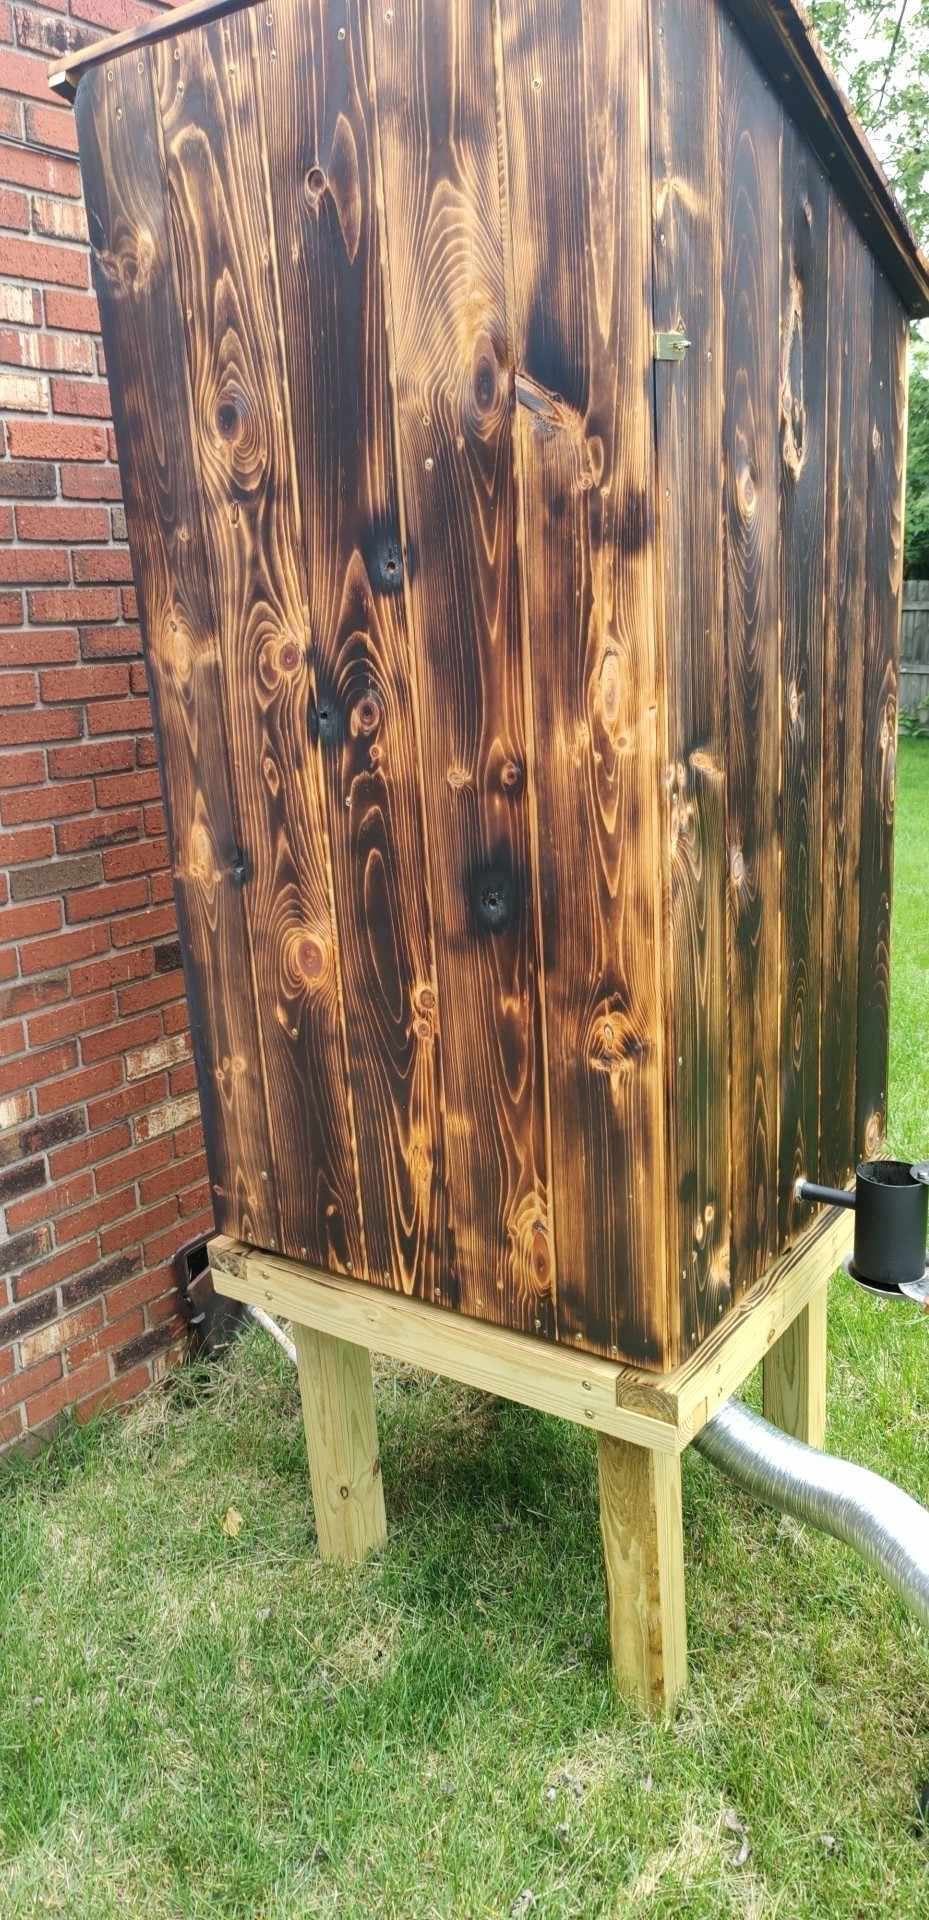
\includegraphics[width=0.45\textwidth]{Figures/Messenger_creation_8ca9e75e-8d85-4b6f-bd27-b4976f07179f.png}
	\caption{The outside of my Smokehouse}
	\label{Smoker}
\end{figure}
\begin{figure}[!htb]
	\centering
	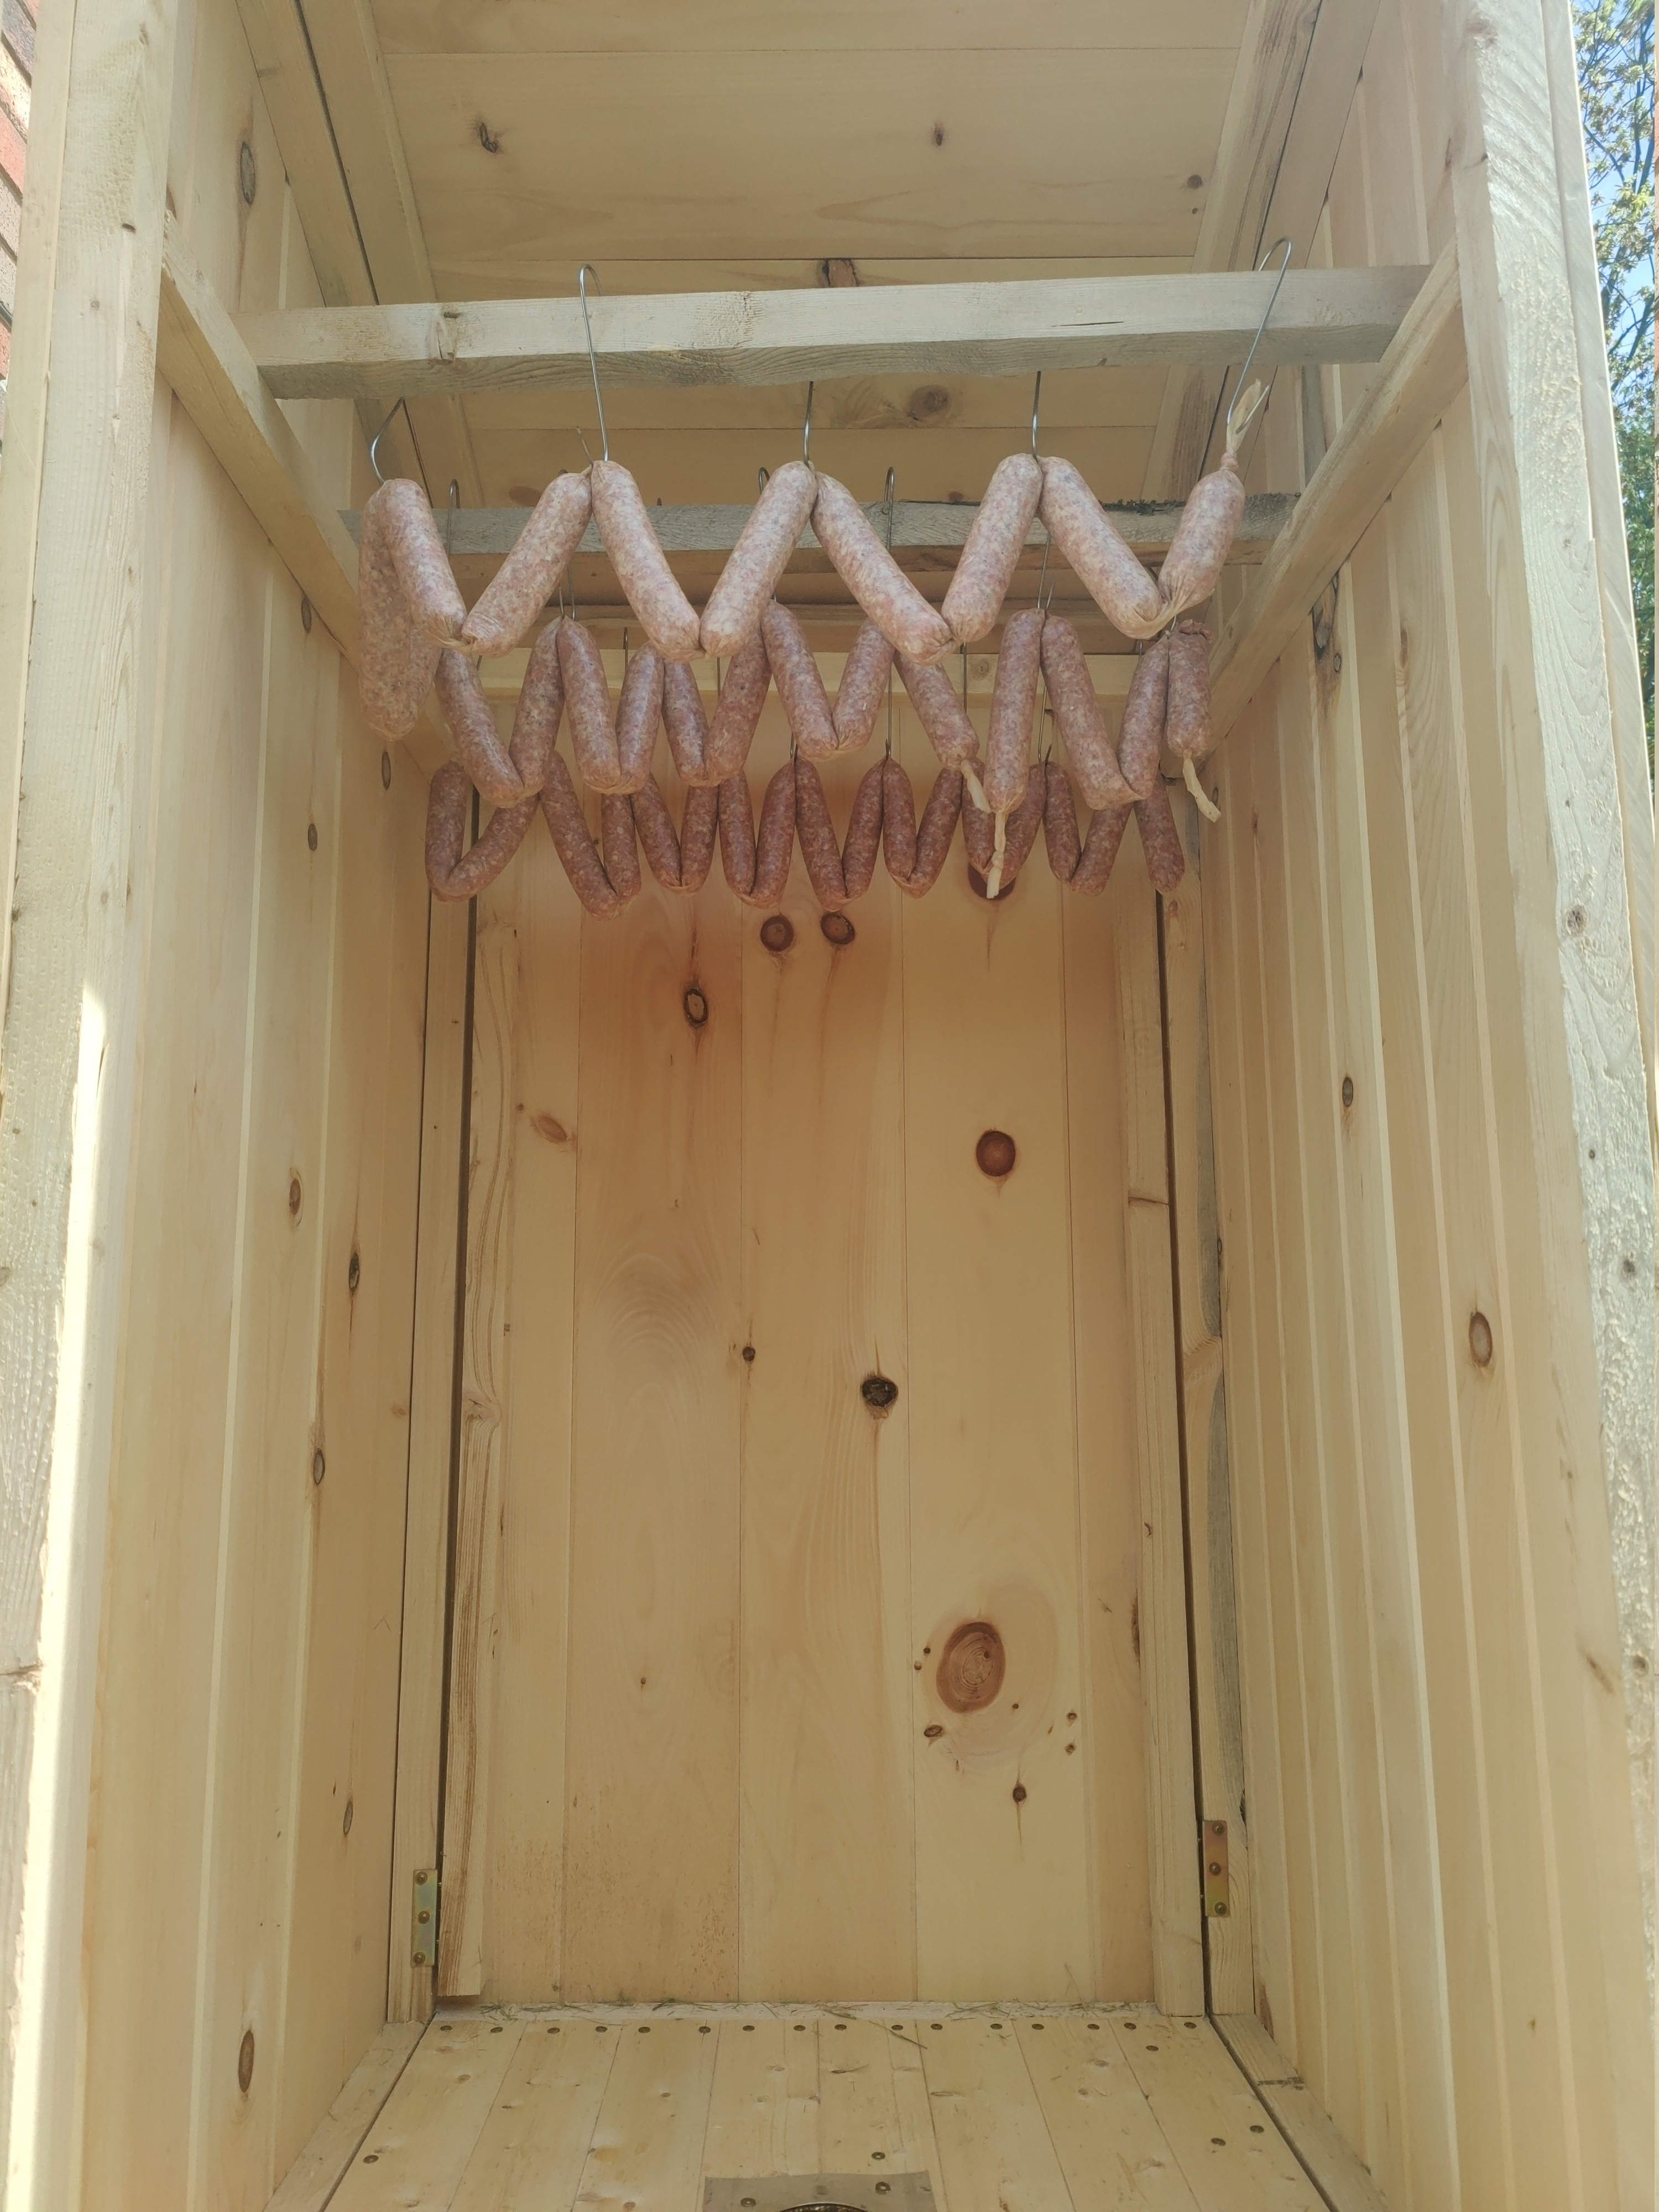
\includegraphics[width=0.45\textwidth]{Figures/2024-04-26-11-13-05-315.jpg}
	\caption{Sausages Smokeing}
	\label{SmokingSausage}
\end{figure}

\subsection{Process of making the sausage}

I broke up the meat into two different batches depending on the method that would be used to break it up. 2kg for grinding and 1.5kg for chopping and beating. TODO:(images of the process for grindig and chopping)

I then added all of the ingredients to each batch scaled to the meat ammounts.


\subsubsection{Chopping and Beating}

I first broke down the pork shoulder, removing the bone first then making thumb sized pieces(Figure \ref{Breakdown}). Once I had reasonably sized pieces I would then use my cleaver to chop the meat until it resembled roughly ground meat(Figure \ref{Chopping}). I could also get a general idea on the progress by the stickiness of the meat as it should get somwhat sticky as it gets processed and the cell walls start to break down. 

Once I wasn't makeing much progress with the knife(and I was getting a sore wrist) I moved on to the large Mortar and Pestle(Figure \ref{MortarPestle}). The mortar and pestle was similar in size and shape to the on found in Figure \ref{MortarIlumination}. I added the various dry ingredients(along with the garlic) and mixed/pounded the sausage mix for a bit. I then added in the required water in a couple of batches and beat until incorporated and back to sticky and not watery/wet. once all of the water was beat in I then beat/pounded it until it had the tackyness that I recognised and could stick to my hand upsidedown (Figure \ref{sticking}).

For the modern grinding I just used my small hobart mixer with the meat grinder attachment with the medium hole plate(about 1/8-3/16in). I then added everything into the bowl and added the ingredients and used the paddle attachment to mix and beat the meat to the required consistency.

 \begin{figure}[!htb]
	\centering
	\includegraphics[width=0.9\textwidth]{Figures/20240524_0088.jpg}
	\caption{Breaking down the pork shoulder}
	\label{Breakdown}
\end{figure}
 \begin{figure}[!htb]
	\centering
	\includegraphics[width=0.9\textwidth]{Figures/20240524\_0097.jpg}
	\caption{Chopping the meat with a cleaver}
	\label{Chopping}
\end{figure}
 \begin{figure}[!htb]
	\centering
	\includegraphics[width=0.9\textwidth]{Figures/20240524_0108.jpg}
	\caption{Pounding the meat with a large Mortar and Pestle}
	\label{MortarPestle}
\end{figure}
\begin{figure}[!htb]
\centering
\includegraphics[width=0.9\textwidth]{Figures/Tacuinum_Sanitatis_p85R.png}
\caption{Example of a mortar and pestle used in period \citep{TacSan}}
\label{MortarIlumination}
\end{figure}
 \begin{figure}[!htb]
	\centering
	\includegraphics[width=0.9\textwidth]{Figures/20240524_0113.jpg}
	\caption{Meat Sticking to upsidedown hand}
	\label{sticking}
\end{figure}

\FloatBarrier

\subsubsection{Stuffing Funnels}

For stuffing the sausage I used two different tools. I used a funnel for the period method and a standard hand crank sausage stuffer for the modern method. The funnel I used was probably a bit small. It worked but was definitly not a speedy or very easy method. If I had a better sized funnel it might have been a bit of a simpler process. The modern stuffer (Figure \ref{stuffer}) I used was much faster(10-20x) as I was able to stuff five of the test sets while switching the casing types in about 10min max. The funnel on the other hand took about 1-2 hours for two test sets.

\begin{figure}[!htb]
	\centering
	\includegraphics[width=0.9\textwidth]{Figures/20240524_0124.jpg}
	\caption{Modern stuffer being used}
	\label{stuffer}
\end{figure}

\subsubsection{Casings}

The casings that I used were both from the the Sausage Maker company. The artificial casings were Collagen casings\footnote{https://www.sausagemaker.com/product/fresh-collagen-casings-32mm/} which are generally made of refined beef hide. They are fully edible and are supposed to mimic the cooking process and "bite" or snap of natural casings. The Natural casings I used were hog casings\footnote{https://www.sausagemaker.com/product/natural-hog-casings-29-32mm/} of a similar size to the artificial casings but had some minor variations due to being from an animal.

\FloatBarrier

\bibliography{bibliography.bib}

\FloatBarrier

\section{Illuminations}\label{b:appendix2}

\begin{figure}[!htb]
	\centering
	\includegraphics[width=0.45\textwidth]{Figures/Amb. 317.2° Folio 59 verso (Mendel I).jpeg}
	\caption{\citep[page 59 Left]{Mendel}}
\end{figure}

\begin{figure}[!htb]
	\centering
	\includegraphics[width=0.45\textwidth]{Figures/Amb. 317.2° Folio 83 verso (Mendel I).jpeg}
	\caption{\citep[page 83 Left]{Mendel}}
\end{figure}

\begin{figure}[!htb]
	\centering
	\includegraphics[width=0.45\textwidth]{Figures/Tacuinum_Sanitatis_p73L.png}
	\caption{\citep[page 73 Left]{TacSan}}
\end{figure}

\begin{figure}[!htb]
	\centering
	\includegraphics[width=0.45\textwidth]{Figures/Tacuinum_Sanitatis_p73R.png}
	\caption{\citep[page 73 Right]{TacSan}}
\end{figure}

\begin{figure}[!htb]
	\centering
	\includegraphics[width=0.45\textwidth]{Figures/Tacuinum_Sanitatis_p74L.png}
	\caption{\citep[page 74 Left]{TacSan}}
\end{figure}

\begin{figure}[!htb]
	\centering
	\includegraphics[width=0.45\textwidth]{Figures/Tacuinum_Sanitatis_p74R.png}
	\caption{\citep[page 74 Right]{TacSan}}
\end{figure}

\begin{figure}[!htb]
	\centering
	\includegraphics[width=0.45\textwidth]{Figures/Tacuinum_Sanitatis_p75L.png}
	\caption{\citep[page 75 Left]{TacSan}}
\end{figure}

\begin{figure}[!htb]
	\centering
	\includegraphics[width=0.45\textwidth]{Figures/Tacuinum_Sanitatis_p75R.png}
	\caption{\citep[page 75 Right]{TacSan}}
\end{figure}

\begin{figure}[!htb]
	\centering
	\includegraphics[width=0.45\textwidth]{Figures/Tacuinum_Sanitatis_p77L.png}
	\caption{\citep[page 77 Left]{TacSan}}
\end{figure}

\begin{figure}[!htb]
	\centering
	\includegraphics[width=0.45\textwidth]{Figures/Tacuinum_Sanitatis_p77R.png}
	\caption{\citep[page 77 Right]{TacSan}}
\end{figure}

\begin{figure}[!htb]
	\centering
	\includegraphics[width=0.45\textwidth]{Figures/Tacuinum_Sanitatis_p78R.png}
	\caption{\citep[page 78 Right]{TacSan}}
\end{figure}

\begin{figure}[!htb]
	\centering
	\includegraphics[width=0.45\textwidth]{Figures/Tacuinum_Sanitatis_p79L.png}
	\caption{\citep[page 79 Left]{TacSan}}
\end{figure}

\begin{figure}[!htb]
	\centering
	\includegraphics[width=0.45\textwidth]{Figures/Tacuinum_Sanitatis_p79R.png}
	\caption{\citep[page 79 Right]{TacSan}}
\end{figure}

\begin{figure}[!htb]
	\centering
	\includegraphics[width=0.45\textwidth]{Figures/Tacuinum_Sanitatis_p82L.png}
	\caption{\citep[page 82 Left]{TacSan}}
\end{figure}

\begin{figure}[!htb]
	\centering
	\includegraphics[width=0.45\textwidth]{Figures/Tacuinum_Sanitatis_p85R.png}
	\caption{\citep[page 85 Right]{TacSan}}
\end{figure}

\end{document}